\documentclass{article}
\usepackage{times}
\usepackage{titlesec}
\usepackage{longtable}
\usepackage{tikz}
\usepackage{wrapfig}
\usepackage{lipsum} 
\usepackage{hhline}
\usepackage{color}
%\usepackage[table]{xcolor}

\usepackage[amssymb]{SIunits}
\usepackage{latexsym}
\usepackage{multirow}
\usepackage{wrapfig}
\usepackage{comment}
\usepackage{import}
\usepackage[ruled, vlined, linesnumbered]{algorithm2e}
\usepackage{amsmath, amsthm, amssymb}
\usepackage{amsfonts}
\usepackage[format=plain,indention=0cm, font=small, labelfont=bf]{caption}
\usepackage{fancyhdr}
%\usepackage[pdftex]{graphicx}
\usepackage[pdftex,
	    colorlinks, 	
	    pdfstartview=FitH,
	    linkcolor=black,
	    citecolor=black,
	    urlcolor=black,
	    filecolor=black
	    ]{hyperref}
\usepackage{lscape}
\usepackage[T1]{fontenc}
\usepackage{floatrow}
\usepackage{enumerate}
\usepackage{pifont}
\usepackage{soul}
\usepackage{esvect}
\usepackage{enumitem}

%\usepackage[dvipsnames]{xcolor}


\usepackage{floatflt}
\usepackage{tabularx}
\usepackage{ragged2e}
\newcolumntype{Y}{ >{\RaggedRight\arraybackslash}X}
\newcommand\T{\rule{0pt}{2.6ex}}      
\newcommand\B{\rule[-1.2ex]{0pt}{0pt}}
\RequirePackage{color}
\definecolor{RED}{rgb}{1,0,0}
\definecolor{BLUE}{rgb}{0,0,1}
\definecolor{White}{rgb}{1,1,1}
\newtheorem{theorem}{Theorem}

%\newcommand{\idx}{CECI}
\newtheorem{thm}{Theorem}
\newtheorem{lem}{Lemma}
%\newtheorem{rule}{Rule}
%\newtheorem{lem}{Lemma}





\newcommand{\sub}{CECI}
\newcommand{\idx}{CECI}
%\newtheorem{example}{Example}
%\newtheorem{lem}{Example}
\newcommand{\simd}{SIMD-X}

\theoremstyle{expln}
\newtheoremstyle{expln}% <name>
{5pt}% <Space above>
{5pt}% <Space below>
{}% <Body font>
{}% <Indent amount>
{\itshape}% <Theorem head font>
{:}% <Punctuation after theorem head>
{}% <Space after theorem headi>
{}% <Theorem head spec (can be left empty, meaning `normal')>
% DOI
%\acmDOI{10.475/123_4}
\newtheorem{expln}{Explain}


%\theoremstyle{rul}
\newtheoremstyle{mystyle}% <name>
{.05in}% <Space above>
{0in}% <Space below>
{\itshape}% <Body font>
{}% <Indent amount>
{\bfseries}% <Theorem head font>
{: }% <Punctuation after theorem head>
{0in}% <Space after theorem headi>
{}% <Theorem head spec (can be left empty, meaning `normal')>
% DOI
%\acmDOI{10.475/123_4}
\theoremstyle{mystyle}
\newtheorem{rul}{Rule}

\newtheoremstyle{taskstyle}% <name>
{.05in}% <Space above>
{0in}% <Space below>
{}% <Body font>
{}% <Indent amount>
{\bfseries}% <Theorem head font>
{.}% <Punctuation after theorem head>
{.1in}% <Space after theorem headi>
{}% <Theorem head spec (can be left empty, meaning `normal')>
% DOI
%\acmDOI{10.475/123_4}
\theoremstyle{taskstyle}
\newtheorem{tstyle}{Research Task}


\definecolor{unitednationsblue}{rgb}{0.36, 0.57, 0.9}
\definecolor{pinkorange}{rgb}{1.0, 0.6, 0.4}
\definecolor{darkseagreen}{rgb}{0.56, 0.74, 0.56}


%\newtheoremstyle{examp}% <name>
%{5pt}% <Space above>
%{5pt}% <Space below>
%{\itshape}% <Body font>
%{}% <Indent amount>
%{\itshape}% <Theorem head font>
%{:}% <Punctuation after theorem head>
%{.5em}% <Space after theorem headi>
%{}% <Theorem head spec (can be left empty, meaning `normal')>
% DOI
%\acmDOI{10.475/123_4}
%\theoremstyle{examp}
%\newtheorem{examp}{Example}
%\newcommand{\td}{{}}
\newcommand{\td}{{\bf\color{red} FIXME~}}
\providecommand{\TODO}[1]{{\protect\color{red}\noindent {\bf [TODO]}\emph{#1} {\bf [/TODO]}}}
\providecommand{\todo}[1]{{\protect\color{red}\noindent {\bf [TODO]}\emph{#1} {\bf [/TODO]}}}
\providecommand{\add}[1]{{\protect\color{red} #1 (ADD) }}
\providecommand{\ADD}[1]{{\protect\color{red} #1 (ADD) }}
\providecommand{\CHECK}[1]{{\protect\color{red} #1 (check) }}
\providecommand{\check}[1]{{\protect\color{red} #1 (check) }}
\providecommand{\DummyText}[1]{{\protect\color{white} #1}}
%\renewcommand{\refname}{References Cited}
\newcommand{\degrees}{$\!\!$\char23$\!$}
\def\rrr#1\\{\par
\medskip\hbox{\vbox{\parindent=2em\hsize=6.12in
\hangindent=4em\hangafter=1#1}}}
\def\baselinestretch{1}

\newcommand\crule[3][black]{\textcolor{#1}{\rule{#2}{#3}}}

%\titlespacing\section{0pt}{1pt plus 0pt minus 2pt}{0pt plus 0pt minus 2pt}
\titlespacing\subsection{0pt}{8pt plus 4pt minus 2pt}{8pt plus 4pt minus 2pt}
%\titlespacing\subsubsection{0pt}{1pt plus 0pt minus 2pt}{0pt plus 0pt minus 2pt}

\newcommand\encircle[1]{%
	\tikz[baseline=(X.base)] 
	\node (X) [draw, shape=circle, inner sep=0, fill=black, text=white] {\strut #1};}
\usepackage{nips_2018}
\usepackage[utf8]{inputenc} % allow utf-8 input
\usepackage[T1]{fontenc}    % use 8-bit T1 fonts
\usepackage{hyperref}       % hyperlinks
\usepackage{url}            % simple URL typesetting
\usepackage{booktabs}       % professional-quality tables
\usepackage{amsfonts}       % blackboard math symbols
\usepackage{nicefrac}       % compact symbols for 1/2, etc.
\usepackage{microtype}      % microtypography
\usepackage{graphicx}
\usepackage[tableposition=top]{caption}
\usepackage{subcaption}
\usepackage{amsmath}
\usepackage{xcolor}

\usepackage{float}
\floatstyle{plaintop}
\restylefloat{table}


\title{ProbabilityCNN: Environment Adaptive Model Without Finetuning}

% The \author macro works with any number of authors. There are two
% commands used to separate the names and addresses of multiple
% authors: \And and \AND.
%
% Using \And between authors leaves it to LaTeX to determine where to
% break the lines. Using \AND forces a line break at that point. So,
% if LaTeX puts 3 of 4 authors names on the first line, and the last
% on the second line, try using \AND instead of \And before the third
% author name.

\author{
  David S.~Hippocampus\thanks{Use footnote for providing further
    information about author (webpage, alternative
    address)---\emph{not} for acknowledging funding agencies.} \\
  Department of Computer Science\\
  Cranberry-Lemon University\\
  Pittsburgh, PA 15213 \\
  \texttt{hippo@cs.cranberry-lemon.edu} \\
  %% examples of more authors
  %% \And
  %% Coauthor \\
  %% Affiliation \\
  %% Address \\
  %% \texttt{email} \\
  %% \AND
  %% Coauthor \\
  %% Affiliation \\
  %% Address \\
  %% \texttt{email} \\
  %% \And
  %% Coauthor \\
  %% Affiliation \\
  %% Address \\
  %% \texttt{email} \\
  %% \And
  %% Coauthor \\
  %% Affiliation \\
  %% Address \\
  %% \texttt{email} \\
}

\begin{document}
% \nipsfinalcopy is no longer used

\maketitle


\begin{abstract}
  We can meet thousands of objects through years, i.e., different kind of animals, plants, and various people, which requires a general model to classify all these objects. On the other hand, in a specific environment, like our home or office, only less than ten objects appear, such as family members, pets, and furniture. Thus a special model recognizing a few objects could be sufficient. Using a special model in these environment could lead automatically to a much higher accuracy since there is a reduction in number of classes. However, using special models has a intrinsic problem that there are so many environment and mind-bogglingly many combinations of objects, which makes it infeasible to train special models one-by-one. In the contrast, the general model could be trained once and used everywhere. General model also has another benefit that it has seen much more images than a special model and a special model derived from the general model could have much higher accuracy than the one trained from scratch. The problem is, given various combination of classes and distribution, could we train a general model and \textit{derive specialized models from it efficiently for all combinations?} The intuitive idea would be transfer learning, in which the the general model is fintuned to adapt for new dataset. However, considering the time latency and energy consumption of finetuning a model, we argue that avoiding fintuning is critical in the efficient derivation of specialied models. Instead, we brought up \textit{probability layer}, which could adapt the general model to all combinations of classes and distribution efficiently without any retraining. Through experiments, it was shown that probability layer without retraining could perform equivalent or even better than transfer learning with retraining.
\end{abstract}


\section{Introduction}
% First paragraph: CNN performs very well at lab setting
Convolutional neural network (CNN) plays an important role in image recognition. In 2012, AlexNet \cite{krizhevsky2012imagenet} achieved a top-5 error of 17\% on ImageNet \cite{deng2009imagenet}, while previous method could only achieve a top-5 error of 25.7\%. Since then, CNNs have become the dominant method and main research direction in image recognition. In 2015, ResNet \cite{he2016deep} achieves a top-5 error of 3.57\%. Considering that the estimated human classification error on ImageNet is 5.1\% \cite{russakovsky2015imagenet}, we can conclude that CNNs have gained the ability of performing better than human. 



% Second paragraph: All of these models are targetting thousands of classes. In a special environment, we only confront less objects.
However, all of these results are gained in lab setting, which overlooks the environment information that we can use in real life. According to our experience, the appearance of classes has strong time and spatial locality. Even if we can meet thousands of objects through years, only less than ten objects would appear in a particular environment, like our home or office. Experiments on videos of day-to-day life from Youtube \cite{shen2017fast} shows that $10$ objects comprised $90$\% of all objects in $85$\% time. While we can train a general model classifying thousands of classes in lab, a special model for tens of objects would be sufficient. This reduction in number of classes could lead to a boost in accuracy automatically. For example, if we randomly guess from $1000$ classes, the accuracy is $0.1\%$, while the accuracy for randomly guess from $10$ classes is $10\%$. In other word, even if we have changed nothing in the model architecture, the reduction in number of classes could naturally provide us a higher accuracy. Thus it is desirable to incorporate the environment information and use a specialized model instead of a general one. The obstacle to this fascinating plan is the mind-bogglingly huge number of specialized scenarios. Considering the combinations of classes, if we take $10$ classes out of $100$ classes, there would be $1.73*10^{14}$ combinations. If class distribution is also taken into consideration, this number could increase further. In order to use specialized models, we much know how to get them efficiently on various combinations of classes and different class distributions. 
% Third paragraph: Transfer learning becomes the dominant method. 
Transfer learning is the dominant method in conquering various problems for implementing CNNs in real world. In transfer learning, we will have a source domain and a target domain. A model will be pretrained on the source domain and the last few layers will be retrained on the target domain such that the model can handle testing data from the target domain. In this process, various problems could be solved, such as lacking training data, using unlabeled data \cite{doersch2015unsupervised, noroozi2016unsupervised}, and allowing quick runtime domain adaption \cite{han2016mcdnn, shen2017fast}. Transfer learning has also shown improvement on accuracy compared with training a model from scratch \cite{oquab2014learning, yosinski2014transferable}, since the model has seen more images in the process of transfer learning. Due to the effectiveness in all these domains, transfer learning has become the method off the top of head. To the best of our knowledge, transfer learning is the only method used to utilize the scenario we described.


% Forth paragraph: Transfer learning needs retraining and shares all problems in training a model from scratch.
Although transfer learning can bring in many benefits, it also has requires expertise in training models and has intrinsic obstacle in automatic retraining. First, the general practice in transfer learning is to freeze the parameters in leading layers and retrain the last few layers, while existing papers \cite{yosinski2014transferable} show that freezing leading layers may have strong negative effect on the accuracy. Without testing various settings, it is hard to know how many layers should be frozen. Second, the choice of training step depends on dataset and a unique setting is hard to find, which makes automatical transfer learning very hard, if not impossible. For example, in the training process of VggNet \cite{simonyan2014very}, a shallow model needs to be trained to initialize the weights in a deeper model and the learning rate is also carefully selected for several times. There is also a long-lasting debate for the best choice of hyper-parameters for various architectures and datasets \cite{bergstra2012random,  glorot2010understanding, he2015delving, smith2017don, wilson2003general}. All of these evidence shows that retraining a model is not a straight forward task and expertise in training process is required, which obstacle the automatical retraining. Third, due to the short time for retraining, the model may not converge and lead to dramatical variance in accuracy, even with the same model and dataset. Given all these intrinsic problems to implement transfer learning in the scenario, a natural question would be whether we can find a method to use the scenario \textit{without retraining}? 

% Fifth paragraph: Rescale has good effect and can replace transfer learning in a scenario.
To use the scenario without retraining, we brought up \textit{probability layer} which can avoid retraining totally and perform better than transfer learning. The benefit are three folds. First, probability layer can make use of the scenario without any retraining, which would save lots of time. Second, probability layer can make prediction based on the knowledge of original model and performs better than training from scratch. Third, through series of experiments, probability layer is shown to have equivalent or even better performance than transfer learning. We argue that probability layer is a better method than transfer learning to make use of various kind of scenarios. 

% Sixth paragraph: Analysis on logits makes our paper different from rescaling
To use probability layer efficiently, the choice of general model is critical and a detailed analysis of logits could predict whether the probability layer will perform well on a general model. Logits is the output of softmax layer which is equipped with almost all the CNNs. Traditional usage of logits is to consider the label with highest logits as the predicted label. Recent works \cite{ba2014deep, bucilua2006model, hinton2015distilling, lopez2015unifying} have shown that logits contain more information beyond that. Actually, logits is critical to the success of probability layer. Through analysis on logits, the selection criteria of the general model is provided and we can predict whether probability layer will work well on a general model without actually running the probability layer.

\section{Related Works}
% Talk about scenario
Many papers have talked about the difference between testing CNN models in lab setting and in the wild. In lab setting, the prevalent benchmarks, like ImageNet \cite{deng2009imagenet} and CIFAR100 \cite{krizhevsky2009learning}, all assumes equal number of images for each class. However, in a more realistic setting \cite{han2016mcdnn, shen2017fast}, different class may have dramatically different frequency and the distribution may also change over time. The question we want to answer is that, given an environment with a number of classes and distribution, how to use this information? All of the existing works \cite{han2016mcdnn, shen2017fast} only use transfer learning to retrain the last few layers, which would introduce huge amount of energy-consumption and time latency. Our method will make use of the distribution efficiently without retraining, thus avoid additional energy-consumption and time latency.

% Unbalanced dataset
Unbalanced dataset focus on the problem that training dataset has different distribution with the testing dataset, which is related to our scenario. One key point of unbalanced dataset is that the minor classes in the training dataset cannot gain same attention as the major classes, thus oversampling on minor classes or undersampling on major classes will be implemented to generate a balanced dataset \cite{wang2016dealing}. Our scenario is different since we assume that we have a model pretrained on balanced dataset and in the testing time the class distribution changes. Another key point of unbalanced dataset is that in the running time, as the distribution changes, the model will keep updating as new inputs come and retraining is constantly needed. Our method avoid retrain at all and could achieve the same or better performance by only changing a few parameters according to the distribution automatically. Thus energy efficiency and speedup could be achieved by our solution.


% Talk about transfer learning
Transfer learning has shown benefit in domain adaption and currently is the dominant method, if not the only one, for domain adaption. To solve the problem that the testing dataset is small, we use transfer learning \cite{oquab2014learning}. To use unsupervised dataset \cite{doersch2015unsupervised, noroozi2016unsupervised}, we use transfer learning. Assume we have a large model handling $1000$ classes and in an environment only $10$ classes appearing, we still use transfer learning \cite{han2016mcdnn, shen2017fast}. Transfer learning has become the only method off the top of head when we consider the change in classes. Although transfer learning shows various benefit, it also has intrinsic shortage residing in the process of training a CNN model. First, it is hard to decide how many layers we should freeze. \cite{yosinski2014transferable} reported that the freezing less layers leads to better performance on different domains and freezing more layers lead to a better performance on similar domains since the co-adapted interactions between layers will be kept. However, it is still hard to decide whether two domains are similar enough and the exact effect of freezing various number of layers. Second, it is hard to decide the hyper-parameters unless actually try different settings. For epoch number, it is hard to predict whether the model will converge or collapse after a fixed number of epochs. The choice of learning rate also depends on both model and dataset. The choice of hyper-parameter need expertise in lab to fine-tune, which is not convenient in a automatical product. Third, the long latency and energy consuming of training a model obstacle the transfer learning on energy-efficient devices, especially in an environment that class number and distributions keep changing. Our method can avoid retraining at all while utilizing the new dataset, thus all the inconvenience related to retraining is avoided naturally.

\section{Probability Layer}
In this section, we introduce the probability layer and the PCNN. Before proceeding further, we introduce the notation that will be used in the rest of the paper.

\textbf{Notation.} A CNN takes as input an image $X$ and outputs a vector of estimated probability for each class \begin{equation}
    \vec{p} = (p_1, p_2, ..., p_n)
\end{equation}
, where $n$ is the number of classes, and select the class with highest estimated probability 
\begin{equation}
    \underset{i}{\text{argmax}} \; p_i
\end{equation}
as the true class. Here we treat the whole CNN model as a classifier which gives the estimated probability $p_i$ for the label i given the input image X
\begin{equation}
    p_i = P(i|X)
\end{equation}. After adding the probability layer, the original prediction $P(i|X)$ will be rescaled and we use $P_t(i|X)$ to denote the rescaled probability. Additionally, we define $P(i)$ and $P_t(i)$ for class distribution in training data and testing data respectively.


\textbf{Key Assumption. } 
% Key assumption
The main difference between proposed layer and the original CNNs is that we take into consideration the environment information. In original CNNs, the prediction for each image will be made individually, assuming a sequence of images is independent and identically distributed (\textit{i.i.d}). However, in real life, this assumption does not hold and strong spatial and temporal locality may exist. In particular, we assume that in the environment the number of classes, class type, and class distribution are fixed while huge difference between training dataset and testing dataset exists. This is a reasonable assumption on environment in real life. Experiments on videos of day-to-day life from Youtube \cite{shen2017fast} shows that $10$ objects comprised $90$\% of all objects in $85$\% time. 

%The prediction will be made by CNNs individually, assuming a sequence of images is independent and identically distributed (i.i.d). In real life, this assumption does not hold and strong spatial and temporal

In this section, we present the \textit{probability layer}. Probability layer is an extra layer after the CNN model, rescaling the output of softmax layer. Rescaling is a topic in statistics \cite{saerens2002adjusting}. To the best of our knowledge, we are the first to discuss rescaling in CNN context. The outputs of original CNNs predict the probability for each class and the probability layer will adjust this prediction based on the difference of class distribution in training and testing dataset. In particular, for classes with different distribution in training and testing dataset, the probability layer will rescale the corresponding outputs from softmax layer according to the difference in distribution. For other classes with same distribution in both training and testing dataset, the outputs of the proposed layer are equal to the outputs of the softmax layer. 


The probability layer will take as inputs the original predicted probability, class distribution in training dataset, as well as the distribution in testing dataset, and output a vector for the rescaled prediction. The first input is the prediction $\vec{P(\cdot|X)}$ from the softmax layer, which represents the original predicted probability for each class from the original CNNs. The second input is a vector of class distribution $\vec{P(\cdot)}$ in training dataset and the third one is a vector of class distribution $\vec{P_t(\cdot)}$ in testing dataset. The probability layer will rescale the predicted probability in $\vec{P(\cdot|X)}$ elementwisely and produce as output a vector $\vec{P_t(\cdot|X)}$ for the rescaled prediction of each class.

Formally, let the outputs of CNNs with and without rescaling are
\begin{equation}
    P_t(i|X) = \frac{P_t(X|i) \cdot P_t(i)}{P_t(x)}
\end{equation}
and
\begin{equation}
    P(i|X) = \frac{P(X|i) \cdot P(i)}{P(x)}
\end{equation}
respectively. Here $P_t(i)$ means the class distribution in testing dataset and $P_t(i|X)$ represents the predicted probability for class $i$ after the probability layer. We assume that $P_t(X|i)$ equals $P(X|i)$ approximately, where $P(X|i)$ is the distribution of image data for class $i$. This assumption makes sense since, for a class $i$, the selection of input x is random. Transforming equation $4$ and $5$ into 
\begin{equation}
    P_t(X|i) = \frac{P_t(i|X) \cdot P_t(X)}{P_t(i)}
\end{equation}
and
\begin{equation}
    P(X|i) = \frac{P(i|X) \cdot P(X)}{P(i)}
\end{equation}
and following our assumption that $P_t(X|i) = P(X|i)$, we can derive that 
\begin{equation}
    P_t(i|X) = \frac{P_t(i)}{P(i)}\cdot P(i|X) \cdot P(X) 
\end{equation}. Considering $\sum_{i=1}^n P_t(i|X) = 1$, we can get that $P(X) = 1/(\sum_{j=1}^{n} \frac{P_t(j)}{P(j)} \cdot P(j|X))$. Finally, the rescaling formular is 
\begin{equation}
    P_t(i|X) = \frac{\frac{P_t(i)}{P(i)} \cdot P(i|X)}{\sum_{j=1}^n \frac{P_t(i)}{P(j)} \cdot P(j|X)}
\end{equation}


To give probability layer the ability of detecting new classes, we choose not to rescale the outputs from softmax layer when original model has strong confidence in its prediction and set the formular of probability layer as
\begin{equation}
    P_t(i|X) = \frac{\frac{P_t(i)}{P(i)} \cdot P(i|X)}{\sum_{j=1}^n \frac{P_t(i)}{P(j)} \cdot P(j|X)} \cdot I_{\{P(i|X) < \omega\}} + P(i|X) \cdot I_{\{P(i|X) >= \omega\}}
\end{equation}
, where $\omega$ is the threshold when we should trust the original prediction and $I_X$ is the indicator function such that
\begin{equation}
I_X(x) = \begin{cases}
1, &\text{if $x \in X$}\\
0, &\text{$o.w.$}
\end{cases}
\end{equation}
. If a model have a strong confidence in its prediction, the accuracy would be much higher than the model's average accuracy. Our experiments show that CNNs will give most of the images high predicted probability and the accuracy of these images will exceed average accuracy a lot. Probability layer helps when the original model is confused on the prediction and will not interfere the decision when the original model has confidence in its prediction.






\begin{figure}[t]
\begin{subfigure}{.25\textwidth}
  \centering
  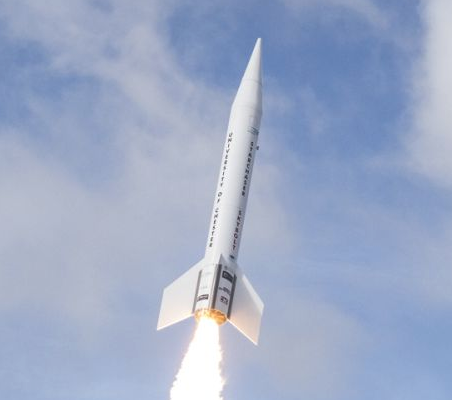
\includegraphics[width=\textwidth]{rocket.png}
  \caption{Rocket}
  \label{fig:sub2}
\end{subfigure}
\begin{subfigure}{.25\textwidth}
  \centering
  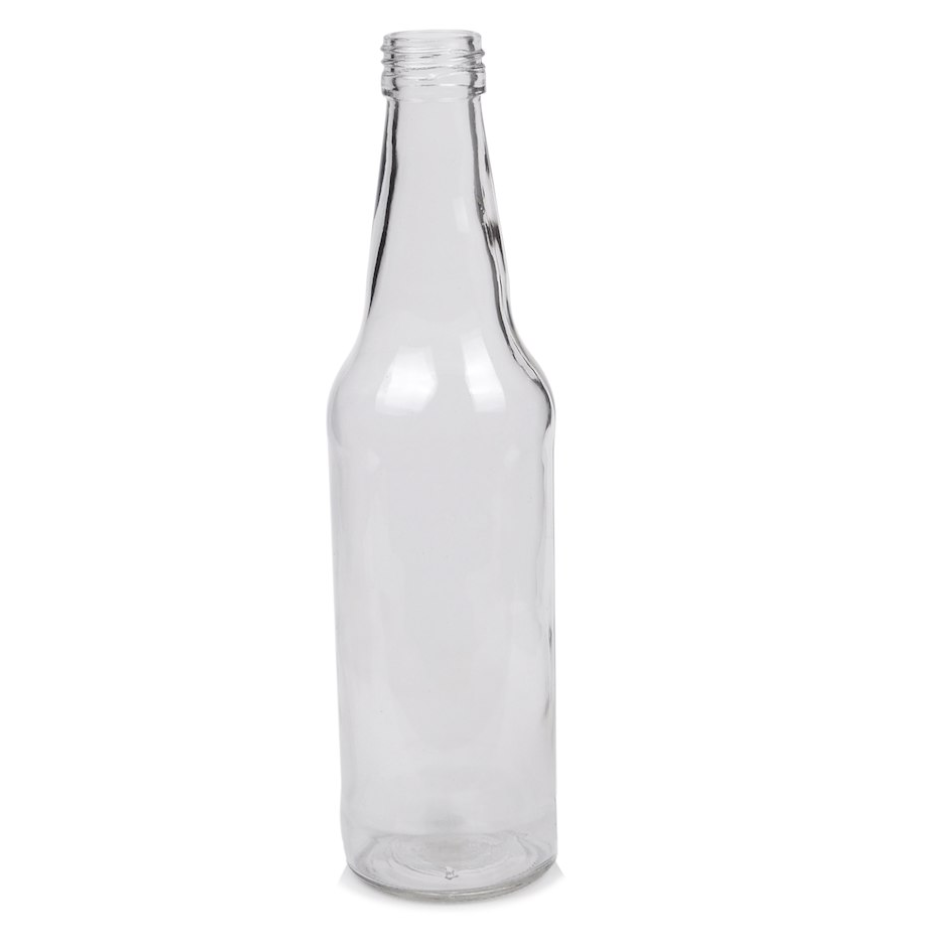
\includegraphics[width=\textwidth]{bottle.png}
  \caption{Bottle}
  \label{fig:sub3}
\end{subfigure}
\begin{subfigure}{.45\textwidth}
  \centering
  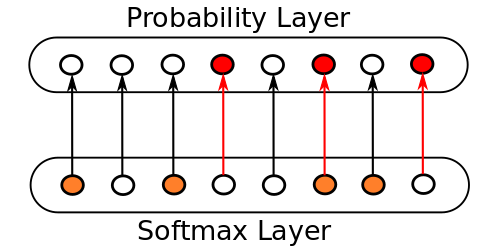
\includegraphics[width=\textwidth]{intuition.png}
  \caption{Computation Intuition}
  \label{fig:sub1}
\end{subfigure}

\caption{Probability Layer Intuition}
\label{fig:intuition}
\end{figure}


% Intuition of probability layer
Probability layer helps by using environment information that original CNNs does not use. When human recognizes an object, both vision and environment information will be used, i.e., what we have seen recently and which objects may appear here. However, CNNs can only make use of vision information while discarding environment information, which makes it extremely difficult to distinguish classes with similar shapes. For example, fig. \ref{fig:sub2} and \ref{fig:sub3} shows images from CIFAR100 for bottle and rocket respectively. It is hard to distinguish these two classes only from images while environment information can easily rule out rocket in most scenarios. 

Fig. \ref{fig:intuition} gives intuition on how probability layer utilize environment information. In fig. \ref{fig:sub1}, the lower row represents the outputs from softmax layer and the upper row represents the probability layer. The orange nodes stand for the classes with high predicted probability in softmax layer and the red nodes stand for the suggestion from environment. The prediction from probability layer will be selected from the intersection of the set of red nodes and orange nodes, which rules out confusing classes for CNNs. 
%how to select general model?


\section{Experiments}
%We use three convolutional neural networks of increasing size and computational complexity: AlexNet \cite{krizhevsky2012imagenet}, ResNet \cite{he2016deep}, and DenseNet \cite{huang2017densely}. We reimplement these three networks on Tensorflow and train the model on CIFAR100 \cite{krizhevsky2009learning} from scratch. The statistics for the original model is shown in Table xxx. In all networks, we attempt to add probability layer after the softmax layer. 

We implemented probability layer on DenseNet \cite{huang2017densely} and evaluated the PCNN on specialized dataset with various number of classes and class distribution. We choose DenseNet as the base model since it is the state-of-the-art and has similar results with other state-of-the-art models, i.e., GoogLeNet \cite{szegedy2015going} and ResNet \cite{he2016deep}. We reimplemented the DenseNet on Tensorflow \cite{abadi2016tensorflow} and trained the model on CIFAR100 \cite{krizhevsky2009learning} from scratch. The \textit{specialized dataset} is generated from CIFAR100 \cite{krizhevsky2009learning}, which originally has $100$ classes with equal weight. 

\textbf{Transfer Learning.} Following the published practice \cite{doersch2015unsupervised, han2016mcdnn, oquab2014learning, shen2017fast, yosinski2014transferable}, all fully-connected layers after convolutional layers are finetuned on generated dataset with same class distribution as the testing dataset. To eliminate the effect of epoch, we used three different epochs, i.e., $1$, $5$, and $30$. The maximum epoch is $30$ because latency and energy efficiency are considered.

To show the potential of PCNN, we evaluate probability layer on specialized datasets composed with various number of classes and class distributions. We begin our experiments by showing that different class combinations have significant influence over the accuracy and probability layer can bring in benefit and perform better than transfer learning on all class combinations. Then we show that probability layer can improve accuracy for any number of classes and make use of unbalanced distribution. We proceed to show that most of the images will have predicted probability higher than $75\%$ and the accuracy among these high-confidence images is $84\%$. Finally, we demonstrate that probability layer is complementary to acceleration methods through combining probability layer with spatial redundancy elimination approach \cite{figurnov2016perforatedcnns} to achieve decreased computation and improved accuracy.

\subsection{Class effect}
We explore the effect of class combinations and compare the performance of probability layer and transfer learning on various class combinations. Fixing number of classes as two, we randomly selected five class combinations and compare the original model, model after transfer learning, and the model with probability layer, see fig. \ref{fig:classEffectExamples}. We see that with the same model, different class combinations may have drmatically different accuracy. While the original model can achieve a accuracy as 83\% for classifying chair and cup, the accuracy for beaver and bear is only 52.5\%. We can also observe that both transfer learning and probability layer can bring in benefit no matter which two classes compose the dataset while probability layer generally performs better than transfer learning. In the randomly selected five class combinations, probability layer can provide an additional benefit of $2.16\%$ on average. Note that for fox and pine, transfer learning provides a slightly better accuracy than probability layer. We believe that this is due to randomness, especially when considering that transfer learning performs better on all other class combinations. 

Fig. \ref{fig:classEffectSummary} gives a summary over performance of all three models on specialized dataset with two and five classes. The figure shows the result from $100$ randomly selected class combinations. We see that, on the original model, while the average accuracy for classifying two classes is $70\%$, the minimum accuracy could be $45\%$ and the maximum accuracy can reach $83\%$, which shows that the accuracy of classifying two classes could change dramatically even using the same model. This observation also holds for transfer learning and probability layer. We can also note that the average accuracy of probability layer is much higher than transfer learning. 

\begin{figure}[t]
    \begin{subfigure}[b]{0.47\textwidth}
        %\centering
        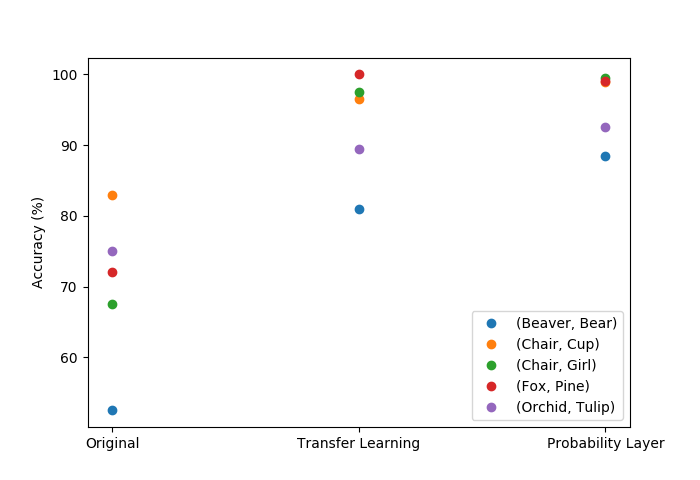
\includegraphics[width=\textwidth]{classEffectLine.png}
        \caption{Concrete examples}
        \label{fig:classEffectExamples}
    \end{subfigure}
    \begin{subfigure}[b]{0.47\textwidth}
        %\centering
        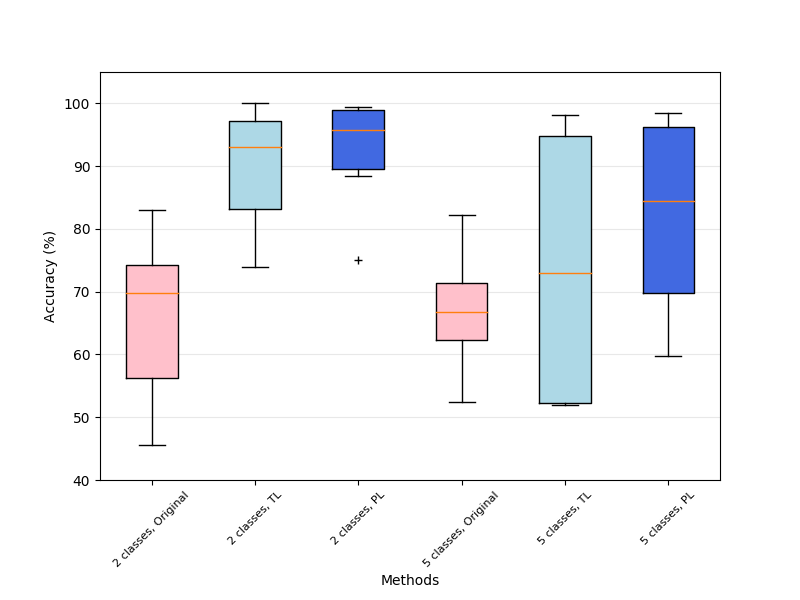
\includegraphics[width=\textwidth]{classEffect.png}
        \caption{Summary of class effect}
        \label{fig:classEffectSummary}
    \end{subfigure}
    \caption{Class effect on the original model, the model after finetuning, and the model with probability layer.} \label{fig:classEffect}
\end{figure}

\subsection{Results on specialized datasets with only majority classes}
% Third paragraph: Experiment setting
We explore probability layer's ability on making use of environment when there are only a few majority classes. For each number of classes, we randomly sampled $100$ subsets of classes and present the average accuracy in fig. \ref{fig:PLvsRetrain}. We see that significant benefit has been achieved by probability layer for all number of classes. When there are 5 classes, an increase more than $20\%$ can be achieved without any finetuning. Another point worth noting is that the benefit diminishes gradually as the number of classes increases. Even if there are $40$ classes, a benefit over $10\%$ could still been observed. This shows significant advantage over previously published results \cite{shen2017fast}, in which no benefit exists when there are more than $15$ classes.
 
We compare our results with transfer learning in fig. \ref{fig:PLvsRetrain}. For every specialized dataset, we finetune the model for $5$ rounds on a training dataset with the same class combinations and class distribution as the testing dataset. For all selected class numbers, probability layer performs better than transfer learning. This advantage of probability layer over transfer learning increases as the number of classes increase. We contribute this phenonmenon to the fact that PCNN has seen more images than transfer learning. Existing papers \cite{yosinski2014transferable} has also reported that transfer learning may destroy the co-adaption between layers and deteriorate the performance on prediction. Another point worth noting is that when the number of classes increases over $90$, retraining would bring worse accuracy than original model without retraining. In contrast, the probability layer can still bring 2\% advantage over original model. We believe the reanson is that the deterioration of co-adaption between layers leads to a decrease in accuracy and the reduction in number of classes cannot make up this deterioration when number of classes is $90$, which is almost same as the original class numbers. Probability layer does not need finetuning and thus avoid this problem. All these observations indicate that probability layer has better ability in using various environment.


\subsection{High confidence, high accuracy}
We justify our design of threshold in probability layer by exhibiting the percentage of images with predicted probability layer higher than various threshold and the accuracy of these images, see fig. \ref{fig:threshold}. While the original denseNet has top-1 accuracy as $73\%$, the accuracy increase to $83\%$ when we set the threshold $\omega$ to be $75\%$. When we increase furtherly the threshold $\omega$ to be $99\%$, the accuracy would increase to $95.01\%$. Thus when a model has strong confidence in its prediction, we should better believe in the model instead of rescaling. 

We also note that a large portion of images can get high predicted probability from original model. For instance, there are more than 60\% images get predicted probability higher than 95\%. For these images that the original model has strong confidence in its prediction, the probability layer will not interfere the decision. The probability layer will step in when the original model is not sure and give suggestion to the probability layer according to the environment information. 


\begin{figure}[!tbp]
\RawFloats

  \centering
  \begin{minipage}[b]{0.49\textwidth}
        \centering
        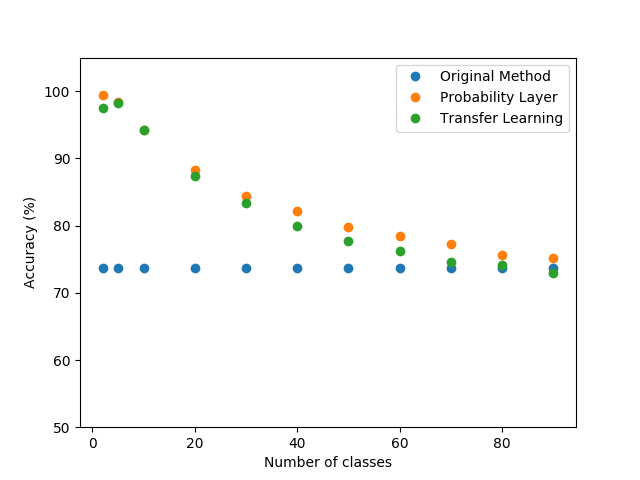
\includegraphics[width=\textwidth]{PLvsRetrain.png}
        \caption{Performance on different number of classes}
        \label{fig:PLvsRetrain}
  \end{minipage}
  \hfill
  \begin{minipage}[b]{0.49\textwidth}
        \centering
        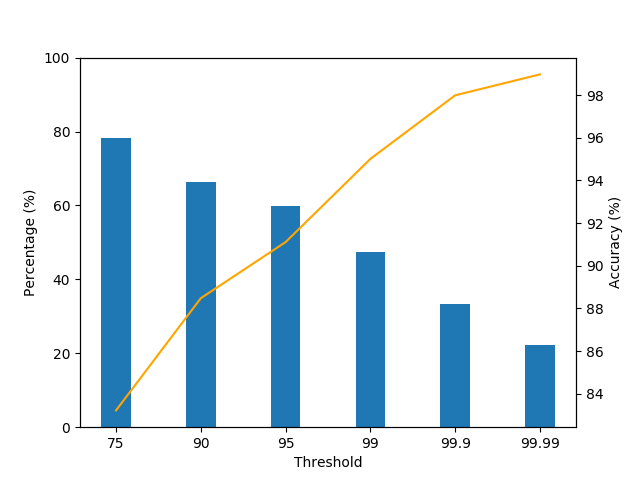
\includegraphics[width=\textwidth]{threshold.png}
        \caption{Threshold}
        \label{fig:threshold}
  \end{minipage}
\end{figure}




\subsection{Results on specialized datasets with both majority and minority classes}

We evaluate the probability layer on noisy environment, in which a few major classes occupies most of the images while a huge number of minority classes also appear. Fig. \ref{fig:variousDistribution5} and fig. \ref{fig:variousDistribution10} shows the results when the numbers of majority classes are five and ten respectively. While the weight of majority classes increases from $50$\% to $100$\%, probability layer performs consistently better than the transfer learning for $5$ or $1$ rounds. Even if we fintune the model for $30$ rounds, probability layer still performs better when weights of major classes is relatively small. When the weights increase further, the advantage of finetuning for $30$ rounds is at most $0.5$\%. Considering the intensive energy-consumption and time latency of retraining for $30$ rounds, this benefit of $0.5$\% advantage is not so significant, especially on devices which requires real time response and has strict energy budget. We should also note that retraining for $1$ rounds would make the accuracy to be much lower than original model when weights of major classes is less than 75\%. Since we need to choose a method before we start in automatically using environment information, we can conclude that probability layer is the most suitable method.

\begin{figure}[t]
    \centering
    \begin{subfigure}[b]{0.49\textwidth}
        \centering
        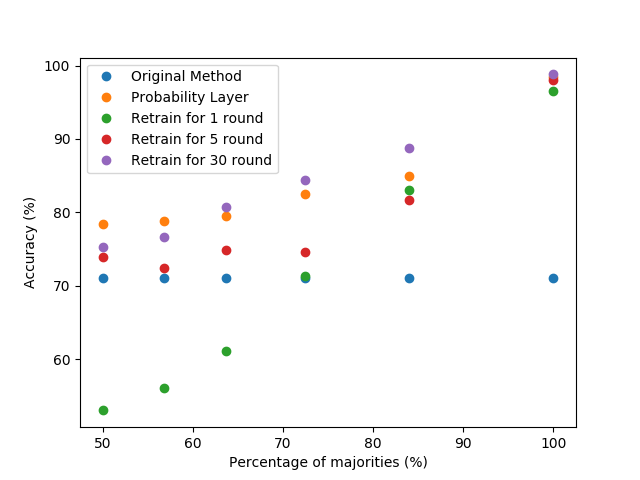
\includegraphics[width=\textwidth]{variousPercentage5.png}
        \caption{Five classes with various distribution}
        \label{fig:variousDistribution5}
    \end{subfigure}
    \begin{subfigure}[b]{0.49\textwidth}
        \centering
        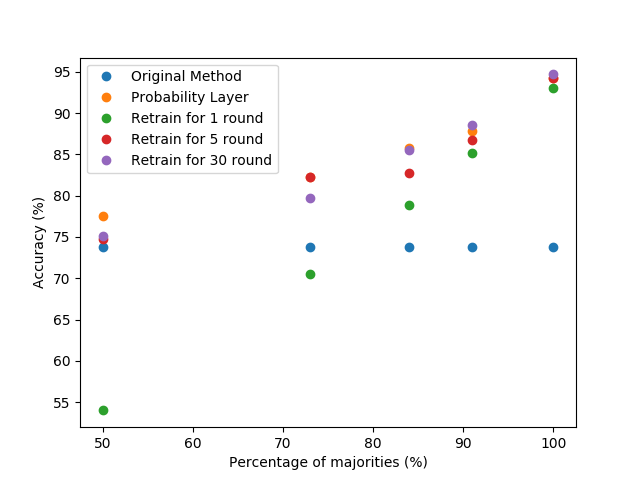
\includegraphics[width=\textwidth]{variousPercentage10.png}
        \caption{Ten classes with various distribution}
        \label{fig:variousDistribution10}
    \end{subfigure}

    \caption{Probability layer on denseNet}\label{fig:complex}
\end{figure}


\subsection{Combining acceleration methods}
A promising way to achieve high speedup and accuracy is to combine acceleration methods with probability layer. For this to succeed, the acceleration methods should utilize different types of redundancy in the network. In this section, we verify that probability layer can be combined with a acceleration methods of using spatial redundancy, \textit{PerforatedCNN} \cite{figurnov2016perforatedcnns}, to achieve high speed up while increasing top-1 accuracy.

We reimplemented the PerforatedCNN \cite{figurnov2016perforatedcnns} on denseNet. PerforatedCNN makes use of spatial redundancy in image by skipping evaluation in some of the spatial positions. Different from other methods in using spatial redundancy, i.e., increasing strides, PerforatedCNN will interpolate these skipped positions using nearest neighborhood, such that the output size will be unchanged. In this way, the architecture remains same and no finetuning is needed. The shortage of PerforatedCNN is that it may introduce a huge decrease in accuracy. Our experiments show that this drawback of PerforatedCNN could be made up by probability layer. Thus combining probability layer with other acceleration methods can both decrease computation and increase accuracy.

We first apply the probability layer to the network. Then we apply the spatial redundancy elimination methods to this network. In the whole process, no finetuning is needed. The PerforatedCNN is tested at the theoretical speedup level of 2x. The testing dataset contains $5$ randomly selected classes with equal frequency. The results are presented in the table \ref{tab:my_label}. Due to class effect, the original model will give a top-1 accuracy of $67.9\%$, which is slightly lower than the average accuracy of DenseNet on CIFAR100. With the probability layer, the model without finetuning can increase the top-1 accuracy dramatically to be $98.4\%$. The PerforatedCNN will give top-1 accuracy of $48.19\%$ if we choose the theoretical speedup level of 2x, which is similar to the results reported in PerforatedCNN \cite{figurnov2016perforatedcnns}. Adding the proposed method, the PerforatedCNN can give a top-1 accuracy of $92.20\%$ while decreasing computation by half, which shows that probability layer complements spatial redundancy elimination methods perfectly and provides a promising perspective of combining probability layer with other acceleration methods.

%Considering that the accuracy of previously published acceleration methods always decrease the accuracy, this combined method shows great potential and 



\begin{table}[h]
    \caption{Summary}
    \label{tab:my_label}

    \centering
    \begin{tabular}{ ccc } 
     Method & Mult. $\downarrow$ & Top-1 Accuracy \\ 
     \hline
     Original Model & 1.0x & 67.79\% \\
     Probability Layer & 1.0x & 98.4\% \\ 
     Perforation & 2.0x & 48.19\% \\ 
     \hline
     Combined Method & 2.0x & 92.20\%
    \end{tabular}
\end{table}




\section{Conclusion}
We have presented probability layer which exploit runtime environment information to increase prediction accuracy. Probability layer requires only a single extra layer after the general CNN models with unnoticable extra computation and obtains a boost in accuracy. Compared to transfer learning, probability layer achieves comparable or even better accuracy boost, avoids retraining, and maintain the ability to detect new classes. Additionally, probability layer can be combined with acceleration methods which exploit various types of network redundancy to achieve further speedups.





\bibliography{nips_2018}
\bibliographystyle{plain}


\end{document}